\documentclass[11pt,twoside,openright]{report}
\usepackage{standalone}
\standalonetrue
\ifstandalone
  \usepackage{../../haziq_thesis}
  \usepackage{../../haziq_maths}
  \usepackage{../../haziq_glossary}
  \addbibresource{../../bib/haziq.bib}
  \externaldocument{../../.texpadtmp/phd-thesis}
\fi

\begin{document}
\hChapterStandalone[1]{Preceding chapters}
\hsetpagenumstandalone{chaptersupp}

%\addcontentsline{toc}{chapter}{Supplementary material}
\renewcommand{\chaptername}{Supplementary}
\setcounter{table}{0}
\renewcommand{\thetable}{S\arabic{chapter}.\arabic{table}}
\setcounter{figure}{0}
\renewcommand{\thefigure}{S\arabic{chapter}.\arabic{figure}}
\setcounter{algorithm}{0}
\renewcommand{\thealgorithm}{S\arabic{algorithm}}
\setcounter{chapter}{0}
\renewcommand{\thechapter}{S\arabic{chapter}}
\setcounter{section}{0}

\chapter{Basic estimation concepts}
\thispagestyle{chaptersone}
\index{frequentist}
Statistics concerns what can be learned from data \citep{davison2003statistical}.
A statistical model comprises of a probabilistic component which drives the data generative process, in addition to a systematic or deterministic component, which sets it apart from pure mathematical models.
Real-valued observations $\by := \{y_1,\dots,y_n\}$ are treated as realisations from an assumed probability distribution with parameters $\theta = (\theta_1,\dots,\theta_p)^\top \in \Theta \subseteq \bbR^p$.
The crux of statistical inference is to estimate $\theta$ given the observed values, so that this optimised value may be used in the model to make deductions.
We describe the \emph{frequentist} and \emph{Bayesian} paradigms for parameter estimation.

\section{Maximum likelihood estimation}

In the frequentist setting, the \emph{likelihood} function, or simply likelihood, is a function of the parameters $\theta$ which measures the plausibility of the parameter value given the observed data to fit a statistical model.
It is defined as the mapping $\theta \mapsto p(\by|\theta)$, where $p(\by|\theta)$ is the probability density function (or in the case of discrete observations, the probability mass function) of the modelled distribution of the observations.
 
\index{maximum likelihood}
\index{likelihood}
\index{log-likelihood}
It is logical to consider the parameter which provides the largest likelihood value,
\begin{equation}\label{eq:ml}
  \hat\theta_{\text{ML}} = \argmax_\theta p(\by|\theta).
\end{equation}
The value $\hat\theta_{\text{ML}}$ is referred to as the \emph{maximum likelihood estimate} for $\theta$.
For convenience, the \emph{log-likelihood} function $L(\theta) = \log p(\by|\theta)$ is maximised instead; as the logarithm is a monotonically increasing function, the maximiser of the log-likelihood function is exactly the maximiser of the likelihood function itself.

\index{gradient!method}
When ML estimates are unable to be found in closed-form, the maximisation problem of \cref{eq:ml} requires iterative, numerical methods to find the maximum.
These methods are often \emph{gradient based}, i.e. algorithms that make use of the gradient of the objective function to be optimised.
Examples include Newton's method, Fisher's scoring, quasi-Newton methods, gradient descent, and conjugate gradient methods.
As the name suggests, these methods require evaluation of gradients or approximate gradients, and in some cases, the Hessian.
Depending on the situation, gradients or Hessians can be expensive or inconvenient to compute or approximate.
In cases of multi-modality of the objective function, the algorithms can potentially converge to a local optima, as it is known that the algorithms are quite sensitive to starting locations.

\index{efficiency}
\index{Cramer-Rao lower bound@Cramér-Rao lower bound}
Besides invariance, the ML estimate comes with the attractive limiting property $\surd{n}(\hat\theta_{\text{ML}} - \theta_{\text{true}}) \xrightarrow{\text{dist.}} \N_p\big(0,\cI(\theta)^{-1}\big)$ \citep{casella2002statistical} as sample size $n\to\infty$, where $\cI(\theta)$ is the Fisher information for $\theta$.
Other asymptotic properties of the ML estimate include consistency, i.e. $\Prob(\Vert \hat\theta_{\text{ML}} - \theta_{\text{true}}\Vert > \epsilon) \xrightarrow{\text{prob.}} 0$ for any $\epsilon>0$, and efficiency, i.e. it achieves the Cramér-Rao lower bound $\Var(\theta_{\text{ML}}) \geq \cI(\theta)^{-1}$.

\index{likelihood ratio test}
As the likelihood measures the plausibility of a parameter value given the data, it can be used to compare two competing models.
Let $\Theta_0 = \{\theta \,|\, \theta_{d+1} = \theta_{d+1,0},\dots,\theta_{p} = \theta_{p,0} \}$ be the set of parameters with restrictions on the last $d$ components of $\theta$.
The \emph{likelihood ratio test} statistic for testing the null hypothesis $\text{H}_0: \theta \in \Theta_0$ against the alternative $\text{H}_1: \theta \notin \Theta_0$ is
\begin{equation}
  \lambda = -2 \log \frac{\sup_{\theta \in \Theta_0} L(\theta)}{\sup_{\theta \in \Theta} L(\theta)} = -2 \big( \log L(\hat\theta_0) - \log L(\hat\theta) \big),
\end{equation}
where $\hat\theta_0 = \argmax_{\theta \in \Theta_0} \log p(\by|\theta)$.
Wilks' theorem states that $\lambda$ has an asymptotic chi-squared distribution with degrees of freedom equal to the number of restrictions  imposed (or rather, the difference in dimensionality of $\Theta$ and $\Theta_0$).
This gives a convenient way of comparing nested models. 

As a remark, models with more parameters will always have higher, or similar, log-likelihood, than models with fewer parameters, because the model has a better ability to fit the data with more free parameters.
In a linear regression setting, this relates to overfitting: a linear model with as many explanatory variables as there are data points ($n=p$) will extrapolate every point in the data set.
Overfitting is an oft cited problem of maximum likelihood.

\section{Bayesian estimation}

\index{subjective Bayes}
\index{objective Bayes}
The \emph{Bayesian} approach to estimating $\theta$ takes a different outlook, in that it supplements what is already known from the data with additional information in the form of prior beliefs about the parameters.
This usually means treating the parameters as random, following some distribution dictated by a \emph{prior density} $p(\theta)$.
There are many ways of categorising different types of priors.
Broadly speaking, priors, and hence Bayesian analysis \citep{robert2007bayesian,kadane2011principles}, can be either \emph{subjective} or \emph{objective}, with the demonyms `subjectivists' and `objectivists' used to refer to those subscribing to each respective principle.
Subjectivists assert that probabilities are merely opinions, while objectivists, in contrast, view probabilities as an extension of logic.
In this regard, objective Bayes seek to minimise the statistician's contribution to inference and ``let data speak for itself'', while subjective Bayes does the opposite.

In either case, inference about the parameters are then performed using the \emph{posterior density}
\begin{equation}
  p(\theta|\by) \propto 
  \myoverbrace{p(\by|\theta)}{\text{likelihood}}
  \times
  \myoverbrace{p(\theta)}{\text{prior}},
\end{equation}
rather than through a single point estimate such as the ML estimate in the frequentist case.
The posterior density encapsulates the uncertainty surrounding the parameters $\theta$ after observing the data $\by$.
The \emph{posterior mean} 
\begin{equation}\label{eq:postmeanest}
  \tilde \theta = \int \theta p(\theta|\by) \dint\theta
\end{equation}
is normally taken to be the point estimate for $\theta$, with its uncertainty usually reported in the form of a \emph{credible interval}: if $\theta_k$ is the $k$'th component of $\theta$, then a $(1-\alpha) \times 100\%$ credible interval for $\theta_k$ is $(\theta_k^l, \theta_k^u)$, where  $\Prob( \theta_k^l \leq \theta_k \leq \theta_k^u ) = (1-\alpha) \times 100\%$.
Under a quadratic loss function, $\tilde\theta$ minimises the expected loss $\E[(\theta - \theta_{\text{true}})^2 ]$ \citep[Sec. 4.4.2, Result 3]{berger2013statistical}, and is hence also viewed as the \emph{minimum mean squared error} (MMSE) estimator.
\index{minimum mean squared error (MMSE) estimate}

\index{MCMC}
On a practical note, integration over the parameter space may be intractable, for instance, the model consists of a large number of parameters for which we would like the posterior mean of, or the marginalising integral cannot be found in closed form.
Markov chain Monte Carlo (MCMC) methods are the standard way of approximating such integrals, by way of random sampling from the posterior.
The sample $\{\theta^{(1)},\dots,\theta^{(T)} \}$ is then manipulated in a way to derive its approximation.
In the case of the posterior mean,
\begin{equation}
  \hat\E[\theta|\by] = \frac{1}{T}\sum_{i=1}^T \theta^{(t)}
\end{equation}
gives an approximation, and its $(1-\alpha) \times 100\%$ credible interval can be approximated using the lower $\alpha/2\times 100\%$ and upper $(1-\alpha/2)\times 100\%$ quantile of the sample.

\index{evidence|see{model evidence}}
\index{model evidence}
The normalising constant is the marginal likelihood over the distribution of the parameters, $p(\by) = \int p(\by|\theta) p(\theta) \dint \theta$.
The quantity $p(\by)$ is also known as the \emph{model evidence}, or simply, \emph{evidence}.
As its name suggests, model evidence is used as a measure of how much support there is for a particular model.
As such, it is used as a basis for model comparison.
Let $p(\by|M_0)$ and $p(\by|M_1)$ be the model evidence for two competing models $M_0$ and $M_1$ respectively.
Define the \emph{Bayes factor} for comparing model $M_0$ against an alternative model $M_1$ as\index{Bayes factor}
\begin{equation}
  \BF(M_0,M_1) = \frac{p(\by|M_0)}{p(\by|M_1)}.
\end{equation}
Values of $\BF(M_0,M_1) < 1$ would suggest that the data provides more evidence for model $M_1$ over $M_0$.

Note that the model evidence is free of $\theta$ because all of the parameters have been marginalised out, or put another way, considered in entirety and averaged over all possible values of $\theta$ drawn from its prior density.
Thus, model comparison using Bayes factors differs from the frequentist likelihood ratio comparison in that it does not depend on any one particular set of values for the parameters.

\section{Maximum a posteriori estimation}

\index{maximum a posteriori estimate|see{MAP estimate}}
\index{MAP estimate}
One may also find the value of $\theta$ which maximises the posterior,
\begin{equation}\label{eq:mapest}
  \hat\theta_{\text{MAP}} = \argmax_\theta p(\by|\theta)p(\theta),
\end{equation}
which is the mode of the posterior distribution.
This quantity is known as the \emph{maximum a posteriori} (MAP) estimate. 
It is different from the ML estimate in that the maximisation objective is augmented with with the prior density for $\theta$.
In this sense, MAP estimation can be seen as regularisation of the ML estimation procedure, whereby a ``penalty'' term is added to avoid overfitting.

MAP estimation is often criticised for not being representative of Bayesian methods.
That is, MAP estimation returns a point estimate with no apparent way of quantifying its uncertainty.
Furthermore, unlike ML estimators, MAP estimators are not invariant under reparameterisation.
If $\theta$ is a random variable with density $p(\theta)$, then the pdf of $\xi := g(\theta)$, where $g:\theta \mapsto g(\theta)$ is a one-to-one transformation, is
\begin{equation}\label{eq:pdftransform}
  p_\xi(\xi) = p_\theta\big(g^{-1}(\xi)\big) \left\vert \frac{\d }{\d \xi} g^{-1}(\xi) \right\vert.
\end{equation}
The second term in \cref{eq:pdftransform} is called the \emph{Jacobian (determinant)}.\index{Jacobian}
Therefore, a different parameterisation of $\theta$ will impact the location of the maximum because of the introduction of the Jacobian into the optimisation objective \cref{eq:mapest}.

\section{Empirical Bayes}

The term \emph{empirical Bayes} \citep{robbins1956empirical,casella1985introduction} refers to a procedure in which features of the prior is informed by the data.
This is realised by parameterising the prior by a hyperparameter $\eta$, i.e. $\theta \sim p(\theta|\eta)$.
%Consider a scenario in which the parameters to be estimated are the mean components of a multivariate normal distribution. 
%It is reasonable to assume that the means were drawn from an identical prior distribution, hyperparameterised by $\eta$.
%%That is, if $\theta = (\theta_1,\dots,\theta_p)^\top$, then $\theta_k|\eta \iid p(\theta_k|\eta)$ for each $k=1,\dots,p$.
%The posterior density for $\theta$ is now written
%\begin{equation}
%  p(\theta|\by) 
%  = \int p(\theta,\eta|\by)p(\eta|\by) \dint\eta
%  = \int \frac{p(\by|\theta)p(\theta|\eta)}{p(\by|\eta)}p(\eta|\by) \dint\eta.
%\end{equation}
%Assuming that the density $p(\eta|\by)$ is concentrated around a point estimate, $\hat\eta = \argmax_\eta p(\eta|\by)$ say, then we can assume that
%\begin{equation}
%  p(\theta|\by) \approx \frac{p(\by|\theta)p(\theta|\hat\eta)}{p(\by|\hat\eta)}.
%\end{equation}
%This approach of optimising the hyperparameters $\eta$ by maximising the 
Values for the hyperparameter are clearly important, because they appear in the posterior for $\theta$: 
\begin{equation}\label{eq:empbayes1}
  p(\theta|\by) = \frac{p(\by|\theta)p(\theta|\eta)}{p(\by|\eta)} 
\end{equation}
To avoid the subjectivist's approach of specifying values for $\eta$ a priori, one instead turns to the data for guidance.
Information concerning $\eta$ is contained in the marginal likelihood $p(\by|\eta) = \int p(\by|\theta)p(\theta|\eta) \dint \theta$.
This paves the way for using the \emph{maximum marginal likelihood} estimate
\begin{equation}
  \hat\eta = \argmax_\eta p(\by|\eta) 
\end{equation}
in place of $\eta$ in the equation of \cref{eq:empbayes1}.
This procedure is also coined \emph{maximum likelihood type-II} \citep{bishop2006pattern}, and is commonly referred to as such in the machine learning literature. \index{maximum likelihood!Type-II}
It is also commonplace in statistics, especially in random-effects or latent variable models which employ a maximum likelihood procedure such as EM algorithm.

As a remark, estimation of $\eta$ itself can be made to conform to Bayesian philosophy, i.e., by placing priors on it and inferring $\eta$ through its posterior.
Such a procedure is referred to as \emph{Bayesian hierarchical modelling}.
A motivation for doing this is because the ML estimate of $\eta$ ignores any uncertainty in it.
Of course, the hyperprior for $\eta$ could be parameterised by a hyper-hyperparameter, and itself have a prior, and so on and so forth.
Evidently the model is specified until such a point where there are parameters of the model which are left unoptimised and must be specified in subjective manner \citep{beal2003variational}.

\chapter{The EM algorithm}\label[supchap]{schap:em}
\thispagestyle{chapterstwo}
\index{EM algorithm}
\index{expectation-maximisation algorithm|see{EM algorithm}}
\index{expectation conditional maximisation algorithm|see{ECM algorithm}}
Often times, there are unobserved, random variables $\bw=\{w_1,\dots,w_n\}$ that are assumed to make up the data generative process, prescribed in the statistical model through the \emph{joint pdf} $p(\by,\bw|\theta)$.
Examples of models that include latent variables are plenty: Gaussian mixture models, latent class analysis, factor models, random coefficient models, and so on.
In order to obtain ML estimates through a direct maximisation of the likelihood, it is necessary to first marginalise out the latent variables via
\begin{equation}\label{eq:varint}
  p(\by|\theta) 
  = \int 
  \myoverbrace{p(\by|\bw,\theta)p(\bw|\theta)}{p(\by,\bw|\theta)}
  \dint \bw
\end{equation}
and obtain the \emph{marginal likelihood}.
Note that the integral is replaced by a summation over all possible values in the case of discrete latent variables $\bw$.
\index{marginal likelihood}

Direct maximisation of the marginal (log-)likelihood might not be favourable due to intractability in obtaining ML solutions.
The form of the marginal likelihood might might not be conducive for closed-form estimates to be found, necessitating the use of numerical, gradient-based methods which is subject to its own undesirable quirks.
Moreover, when the evaluation of the (log-)likelihood, gradient and/or Hessian are expensive to compute, then numerical methods are burdensome to execute.

It is usually the case that if the latent variables $\bw$ were somehow known, estimation would be made simpler.
That is, the solution to $\argmax_\theta \log p(\by,\bw|\theta)$ can be obtained in a simple manner.
The expectation-maximisation algorithm \citep{dempster1977maximum}, commonly known as the EM algorithm, is an iterative procedure which exploits the fact that the so-called \emph{complete data likelihood} is easier to work with.
Correspondingly, in EM terminology, the marginal likelihood is referred to as the \emph{incomplete data likelihood}.
\index{log-likelihood!complete data}
\index{log-likelihood!incomplete data}

We describe a derivation of both a general EM algorithm and an EM algorithm for models whose data generative pdf belongs to an exponential family of pdfs. 
Interestingly, the EM algorithm can be modified to obtain maximum a posteriori estimates or penalised log-likelihood solutions.
As a note, the EM algorithm is not an algorithm per se, in that it does not provide exact instructions as to what the E- and M-steps should comprise of.
Rather, it is a generic device to obtain parameter estimates \citep{mclachlan2007algorithm}.

\section{Derivation of the EM algorithm}

For want of an iterative procedure to obtain maximum likelihood estimates, we seek a solution to 
\begin{equation}\label{eq:em1}
  \argmax_\theta \{ L(\theta|\by) - L(\theta^{(t)}|\by) \geq 0 \},
\end{equation}
where the solution to \cref{eq:em1} yields an improvement to the current $t$'th iteration of the log-likelihood value $L(\theta^{(t)}|\by)$.
Note that the objective function in \cref{eq:em1} forms an upper bound for the quantity $Q(\theta|\theta^{(t)})$, as shown below:
\begin{align*}
  L(\theta|\by) - L(\theta^{(t)}|\by)
  \phantom{:}={}& \log \int p(\by|\bw,\theta)p(\bw|\theta) \, \frac{p(\bw|\by,\theta^{(t)})}{p(\bw|\by,\theta^{(t)})}  \dint\bw - \log p(\by|\theta^{(t)}) \\
  \phantom{:}\geq{}& \int p(\bw|\by,\theta^{(t)}) \log \frac{p(\by|\bw,\theta)p(\bw|\theta)}{p(\bw|\by,\theta^{(t)})} \dint\bw \mycomment{(Jensen's inequality)} \\
  \phantom{:}& - \log p(\by|\theta^{(t)})\int p(\bw|\by,\theta^{(t)}) \dint \bw \\
  \phantom{:}={}& \int p(\bw|\by,\theta^{(t)}) \log \frac{p(\by|\bw,\theta)p(\bw|\theta)}{p(\bw|\by,\theta^{(t)})p(\by|\theta^{(t)})} \dint\bw\\
  =:{}& Q(\theta|\theta^{(t)}).
\end{align*}
Evidently, to maximise $L(\theta|\by)$, we can't do any worse than maximising $Q(\theta|\theta^{(t)})$ in $\theta$.
Denote by $\theta^{(t+1)}$ as the maximiser of $Q(\theta|\theta^{(t)})$. 
Then,
\begin{align*}
  \theta^{(t+1)}
  &= \argmax_\theta \int p(\bw|\by,\theta^{(t)}) \log \frac{p(\by|\bw,\theta)p(\bw|\theta)}{p(\bw|\by,\theta^{(t)})p(\by|\theta^{(t)})} \dint\bw \\
  &= \argmax_\theta \int p(\bw|\by,\theta^{(t)}) \log p(\by|\bw,\theta)p(\bw|\theta) \dint\bw \\
  &= \argmax_\theta \int p(\bw|\by,\theta^{(t)}) \log p(\by,\bw|\theta) \dint\bw \\
  &= \argmax_\theta \E_\bw \left[\log p(\bw,\by|\theta) | \by, \theta^{(t)} \right] 
\end{align*}
We arrive at an iterative procedure summarised succintly as the following:

\begin{algorithm}[H]
\caption{EM algorithm}\label{alg:EM4}
\begin{algorithmic}[1]
  \State \textbf{initialise} $\btheta^{(0)}$ and $t\gets 0$
  \While{not converged}
    \State E-step: compute $Q(\theta|\theta^{(t)}) = \E_\bw \left[\log p(\bw,\by|\theta) | \by, \theta^{(t)} \right]$
    \State M-step: $\theta^{(t+1)} \gets \argmax_\theta Q(\theta|\theta^{(t)})$
    \State $t \gets t + 1$
  \EndWhile
\end{algorithmic}
\end{algorithm}

\vspace{-0.9em}
Notice that the log-likelihood function satisfies
\begin{equation}
  L(\theta|\by) \geq L(\theta^{(t)}|\by) + Q(\theta|\theta^{(t)}),
\end{equation}
for which equality is achieved when $\theta = \theta^{(t)}$, since
\begin{align*}
  Q(\theta^{(t)}|\theta^{(t)})
  &= \int p(\bw|\by,\theta^{(t)}) \log \frac{p(\by|\bw,\theta^{(t)})p(\bw|\theta^{(t)})}{p(\bw|\by,\theta^{(t)})p(\by|\theta^{(t)})} \dint\bw \\
  &= \int p(\bw|\by,\theta^{(t)}) \cancelto{0}{\log \frac{p(\by,\bw|\theta^{(t)})}{p(\by,\bw|\theta^{(t)})}} \dint\bw\\
  &=0.
\end{align*}
This implies that the EM algorithm improves the log-likelihood values at each iteration, since
\begin{align*}
  L(\theta^{(t+1)}|\by) - L(\theta^{(t)}|\by) \geq  Q(\theta^{(t+1)}|\theta^{(t)}) \geq 0
\end{align*}
and $Q(\theta^{(t+1)}|\theta^{(t)}) \geq Q(\theta^{(t)}|\theta^{(t)}) = 0$ since $\theta^{(t+1)}$ maximises $Q(\cdot|\theta^{(t)})$.

The expectation in the E-step involves the conditional pdf $p(\bw|\by,\theta^{(t)})$.
Viewed through a Bayesian lens, this is the posterior density of the latent variables using the $t$'th iteration parameter values.
The success of the E-step is predicated on the availability of the conditional pdf for the expectation.
If not, approximations to the E-step can be explored, for example using Monte Carlo methods \citep{wei1990monte} or a variational approximation \citep{beal2003variational}.

The solution to the M-step usually, but not always, exists in closed form.
Maximising the $Q$ function over all possible values of $\theta$ may not be feasible \citep{mclachlan2007algorithm}.
In such situations, the generalised EM algorithm (as defined by \cite{dempster1977maximum}) requires only that $\theta^{(t+1)}$ be chosen in a way that
\[
  Q(\theta^{(t+1)}|\theta^{(t)}) \geq Q(\theta^{(t)}|\theta^{(t)}).
\]
That is, $\theta^{(t+1)}$ is chosen so as to increase the value of the $Q$ function at its current parameter value.
As seen in the argument above, this requirement is sufficient for a guaranteed increase in the log-likelihood function at each iteration.


\section{Exponential family EM algorithm}
\label{apx:expem}
\index{EM algorithm!exponential family}

Consider the density function $p(\cdot|\btheta)$ of the complete data $\bz = \{\by,\bw\}$, which depends on parameters $\btheta = (\theta_1,\dots,\theta_s)^\top \in\Theta\subseteq\bbR^s$, belonging to an exponential family of distributions.
This density takes the form $p(\bz|\btheta) = B(\bz) \exp \big( \ip{\bfeta(\btheta), \bT(\bz)} -  A(\btheta) \big)$, where $\bfeta:\bbR^s \mapsto \bbR$ is a link function,  $\bT(\bz) = \big(T_1(\bz),\dots,T_s(\bz)\big)^\top \in \bbR^s$ are the sufficient statistics of the distribution, and $\ip{\cdot,\cdot}$ is the usual Euclidean dot product.
It is often easier to work in the \emph{natural parameterisation} of the exponential family distribution \index{exponential family distribution}
\begin{align}\label{eq:pdfexpfamnat}
  p(\bz|\bfeta) = B(\bz) \exp \big( \ip{\bfeta, \bT(\bz)} -  A^*(\bfeta) \big)
\end{align}
by defining $\bfeta := \big(\eta_1(\btheta),\dots,\eta_r(\btheta)\big) \in \cE$, and $\exp A^*(\bfeta) = \int B(\bz) \, \exp \, \ip{\bfeta, \bT(\bz)}  \dint \bz$ to ensure the density function normalises to one.
As an aside, the set $\cE := \big\{ \bfeta = (\eta_1,\dots,\eta_s) \,|\, \int  \exp A^*(\bfeta) < \infty \big\}$ is called the \emph{natural parameter space}.
If $\dim \cE = r < s = \dim \Theta$, then the the pdf belongs to the \emph{curved exponential family} of distributions.
If $\dim \cE = r = s = \dim \Theta$, then the family is a \emph{full exponential family}.

Assuming the latent $\bw$ variables are observed and working with the natural parameterisation, then the complete maximum likelihood (ML) estimate for $\bfeta$ is obtained by solving 
\begin{align}\label{eq:expEM1}
  \frac{\partial}{\partial\bfeta}\log p(\bz|\bfeta)
  &= \bT(\bz) - \frac{\partial}{\partial\bfeta} A^*(\bfeta) = 0.
\end{align}
Of course, the variable $\bw$ are never observed, so the ML estimate for $\bfeta$ can only be informed from what is observed.
Let $p(\by|\bfeta) = \int p(\by,\bw|\bfeta) \dint \bw$ represent the marginal density of the observations $\by$.
Now, the ML estimate for $\bfeta$  is obtained by solving
\begin{align}
  \frac{\partial}{\partial\bfeta}\log p(\by|\bfeta)
  &= \frac{1}{p(\by|\bfeta)} \cdot \frac{\partial}{\partial\bfeta}  p(\by|\bfeta) \nonumber \\
  &= \frac{1}{p(\by|\bfeta)} \cdot \frac{\partial}{\partial\bfeta} \left( \int p(\by,\bw|\bfeta) \dint \bw \right) \nonumber \\
  &= \frac{1}{p(\by|\bfeta)}  \int \left( \frac{\partial}{\partial\bfeta} p(\by,\bw|\bfeta) \right) \dint \bw \nonumber \\
  &= \frac{1}{p(\by|\bfeta)}  \int \left( p(\by,\bw|\bfeta) \frac{\partial}{\partial\bfeta} \log p(\by,\bw|\bfeta) \right) \dint \bw \nonumber \\
  &= \int \left( \bT(\by,\bw) - \frac{\partial}{\partial\bfeta} A^*(\bfeta) \right) p(\bw|\by,\bfeta) \dint \bw \nonumber \\
  &= \E_\bw \big[ \bT(\by,\bw) | \by \big] - \frac{\partial}{\partial\bfeta} A^*(\bfeta) \label{eq:expEM2}
\end{align}
equated to zero.
Note that we are allowed to change the order of integration and differentation provided the integrand is continuously differentiable.
So the only difference between the first order condition of \cref{eq:expEM1} and that of \cref{eq:expEM2} is that the sufficient statistics involving the unknown $\bw$ are replaced by their conditional or posterior expectations.
%but this is not an issue: by the law of total expectations, $\E\bT(\bz) = \E \bT(\by,\bw) = \E \big[ \E_\bw[\bT(\by,\bw)|\by] \big]$
%so solving $\bT(\bz) = \E \bT(\bz)$ for $\btheta$ is not possible without some manipulation.

A useful identity to know is that $\frac{\partial}{\partial\bfeta} A^*(\bfeta) = \E_\bz[ \bT(\bz)]$ \citep[Thm. 3.4.2 \& Exer. 3.32(a)]{casella2002statistical}, which can be expressed in terms of the original parameters $\btheta$.
As a consequence, solving for the ML estimate for $\btheta$ from the FOC equations \cref{eq:expEM2} is possible without having to deal with the derivative of $A^*$ with respect to the natural parameters.
Having said this, an analytical solution in $\btheta$ may not exist, because the relationship of $\btheta$ could be implicit in the set of equations $\E_\bw \big[ \bT(\bw,\by) | \by, \btheta \big] = \E_{\by,\bw}\left[ \bT(\by,\bw) | \btheta \right]$.
One way around this is to employ an iterative procedure, as detailed in \cref{alg:EM3}.

\begin{algorithm}[hbt]
\caption{Exponential family EM}\label{alg:EM3}
\begin{algorithmic}[1]
  \State \textbf{initialise} $\btheta^{(0)}$ and $t\gets 0$
  \While{not converged}
    \State E-step: $\tilde\bT^{(t+1)}(\by,\bw) \gets \E_\bw \big[ \bT(\bw,\by) | \by, \btheta^{(t)} \big]$
    \State M-step: $\btheta^{(t+1)} \gets$ solution to $\tilde\bT^{(t+1)}(\by,\bw) = \E_{\by,\bw}\left[ \bT(\by,\bw) | \btheta \right]$
    \State $t \gets t + 1$
  \EndWhile
\end{algorithmic}
\end{algorithm}

To see how \cref{alg:EM3} motivates the EM algorithm, consider the following argument.
Recall that for the EM algorithm, the function $Q_t(\bfeta) = \E_\bw[\log p(\by,\bw|\bfeta) | \by,\bfeta^{(t)}]$ is maximised at each iteration $t$.
For exponential families of the form \cref{eq:pdfexpfamnat}, the $Q_t$ function turns out to be
\[
 Q_t(\bfeta) = \E_\bw \big[ \ip{\bfeta, \bT(\bz)} | \by,\bfeta^{(t)} \big] -  A^*(\bfeta) + \log B(\bz),
\]
and this is maximised at the value of $\bfeta$ satisfying
\begin{align*}
  \frac{\partial}{\partial\bfeta} Q_t(\bfeta)
  &= \E_\bw \big[ \bT(\by,\bw) | \by,\bfeta^{(t)} \big] - \frac{\partial}{\partial\bfeta}A^*(\bfeta) = 0,
\end{align*}
a similar condition to \cref{eq:expEM2} when obtaining ML estimate of $\bfeta$.
Thus, $Q_t$ is maximised by the solution to line 4 in  \cref{alg:EM3}.

\section{Bayesian EM algorithm}
\index{EM algorithm!Bayesian}

A simple modification of the EM algorithm can be done to obtain maximum a posteriori estimates, or maximum penalised likelihood estimates.
Under a Bayesian framework, a prior is assigned on the model parameters, $\theta\sim p(\theta)$.
Recall that the MAP estimate is obtained as the maximiser of the log-density $\log p(\by|\theta) + \log p(\theta)$.
%\begin{equation}
%  \log p(\by|\theta) + \log p(\theta).
%\end{equation}

The EM algorithm works as before, but replaces the E-step with 
\begin{equation}\label{eq:bayesem}
  \E_\bw \left[\log p(\bw,\by|\theta) + \log p(\theta) | \by, \theta^{(t)} \right]
  = Q(\theta|\theta^{(t)}) + \log p(\theta)
\end{equation}
since $\log p(\theta)$ has no terms involving the latent variables $\bw$.
The M-step now maximises \cref{eq:bayesem} with respect to $\theta$, which includes the log prior density (or a penalty term).
It would seem that the regular EM algorithm maximises \cref{eq:bayesem} such that $p(\theta) \propto \const$ is a diffuse prior for $\theta$.
\citet{beal2003} discuss a more Bayesian extension of EM, in which the output of the so-called \emph{variational Bayes EM} algorithm are (approximate) posterior distributions of the parameters, rather than MAP estimates discussed here.



\chapter{Hamiltonian Monte Carlo}\label[supchap]{misc:hmc}
\thispagestyle{chaptersfour}
%\section{A brief introduction}
\label{misc:hmc}

Hamiltonian Monte Carlo had its beginnings in statistical physics, with the \citeyear{duane1987hybrid} paper by \citeauthor{duane1987hybrid} using what they called `Hybrid Monte Carlo' in lattice models of quantum theory.
Their work merged the approaches of molecular dynamics and Markov chain Monte Carlo methods.
As interesting side note, their method abbreviates also to `HMC', but throughout the statistical literature, it is more commonly referred to by its more descriptive name Hamiltonian Monte Carlo.
Incidentally, the use of HMC started with applications to neural networks as early as 1996 (see \citet{neal2011mcmc} for an excellent review of the subject matter).
It was not until 2011 when active development of the method, and in particular, software for for statistical applications began.
The \proglang{Stan} initiative \citep{carpenter2016stan} began in response to difficulties faced when performing full Bayesian inference on multilevel generalised linear models.
These difficulties mainly involved poor efficiency in usual MCMC samplers, particularly high autocorrelations in the posterior chains, which meant that many chains and many iterations were required to get an adequate sample.
It was a case of exhausting all possible algorithmic remedies for existing samplers (Gibbs samplers, Metropolis samplers, etc.), and realising that fundamentally not much improvement can be had unless a novel sampling technique was discovered.

The basic idea behind HMC is to use Hamiltonian dynamics to propose new states in the posterior sampling, rather than relying on `random walks'.
If one were to understand and use the geometry of the posterior density to one's benefit, then it should be possible to generate new proposal states with high probabilities of acceptance and move far away from the current state.
Hamiltonian dynamics, like classical Newtonian mechanics, provides a framework for modelling the motion of a body in space across time $t$. 
Additionally, Hamiltonian dynamics concatenates the position vector $x$ with its momentum $z$, and the motion of $x$ in $d$-dimensional space is then described through Hamilton's equations
\begin{equation}\label{eq:hamilton1}
  \frac{\d x}{\d t} = \frac{\partial H}{\partial z}
  \hspace{0.5cm}\text{and}\hspace{0.5cm}
  \frac{\d z}{\d t} = -\frac{\partial H}{\partial x},
\end{equation}
where $H=H(x,z)$ is called the Hamiltonian of the system.
The Hamiltonian is an operator which encapsulates the total energy of the system.
In a closed system, one can express the sum of operators corresponding to the kinetic energy $K(p)$ and the potential energy $U(z)$ of the system
\begin{equation}\label{eq:hamilton2}
  H(x,z) = K(z) + U(x).
\end{equation}
Substituing \cref{eq:hamilton2} into \cref{eq:hamilton1}, we get the system of partial differential equations (PDEs)
\begin{equation}\label{eq:hamilton3}
  \frac{\d x}{\d t} = \frac{\partial}{\partial z} K(z)
  \hspace{0.5cm}\text{and}\hspace{0.5cm}
  \frac{\d z}{\d t} = -\frac{\partial}{\partial x}U(x).
\end{equation}

To describe the evolution of $\big(x(t),z(t)\big)$ from time $t$ to $t+T$, it is necessary to discretise time, and split $T = L\epsilon$.
The quantity $L$ is known as the number of \emph{leapfrogs}, and $\epsilon$ the \emph{step size}.
\begin{center}
  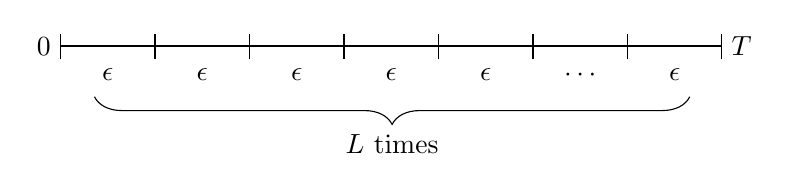
\begin{tikzpicture}[xscale=1.2, yscale=0.8]
    \draw [thick]  (0,0) -- (7,0);
    \foreach \x in  {0,1,2,3,4,5,6,7}
    \draw (\x,-.2) -- (\x, .2);
    \foreach \x in  {0.5,1.5,2.5,3.5,4.5}
    \node[align=center, below] at (\x,-.2) {$\epsilon$};
    \node[align=center, below] at (5.5,-.2) {$\cdots$};
    \node[align=center, below] at (6.5,-.2) {$\epsilon$};
    \node[align=center, left] at (0,0) {$0$};
    \node[align=center, right] at (7,0) {$T$};
    \draw[decorate, decoration={brace, mirror, amplitude=10pt}, xshift=-4pt, yshift=0pt]
    (0.5,-0.8) -- (6.8,-0.8) node [midway,below,yshift=-10pt] {$L$ times};
  \end{tikzpicture}
\end{center}
The system of PDEs is solved using Euler's method, or the more commonly used leapfrog integration, which is a three-step process:
\begin{table}[H]
  \centering
  \begin{tabular}{lrl}
    1. \textbf{Half-step momentum.} 
    &$z(t + \epsilon/2) =$ 
    &\hspace{-7pt}$z(t) - \frac{\epsilon}{2} \, \frac{\partial}{\partial x} U \big( x(t) \big)$ \\[0.6em]
    2. \textbf{Full-step position.} 
    &$x(t + \epsilon) =$ 
    &\hspace{-7pt}$x(t) + \epsilon \, \frac{\partial}{\partial  z} K \big(  z(t + \epsilon / 2) \big)$ \\[0.6em]
    3. \textbf{Half-step momentum.} 
    &$z(t + \epsilon) =$ 
    &\hspace{-7pt}$z(t + \epsilon/2) =  z(t) - \frac{\epsilon}{2} \, \frac{\partial}{\partial x} U \big( x(t) \big)$ \\[0.6em]
  \end{tabular}
\end{table}
\vspace{-1.5em}
\noindent in which steps 1--3 are repeated $L$ times.

Having knowing the formula for how particles move in space, we can use this information to treat random points drawn from some probability density as `particles'.
Randomness of position and momentum are prescribed through probability densities on each.
Given some energy function $E(\theta)$ over states $\theta$, the \emph{canonical distribution} of the states $\theta$ (otherwise known as the \emph{canonical ensemble}) is given by the probability density function
\[
  p(\theta) \propto \exp \left( -\frac{E(\theta)}{k\tau} \right),
\]
where $k$ is Boltzmann's constant, $\tau$ is the absolute temperature of the system.
The Hamiltonian is one such energy function over states $(x,z)$.
By replacing $E(\theta)$ by \cref{eq:hamilton2} in the pdf above, we realise that the distribution for $x$ and $z$ are independent.
The system can be manipulated such that $k\tau=1$---in any case, these are constants which can be absorbed into one of the terms in the pdf anyway.

Using a \emph{quadratic kinetic energy} function $K(z) = z^\top M^{-1} z/2$\footnotemark, we find that the probability density function for $z$ is
\[
  p(z) \propto \exp \left(-\half z^\top M^{-1} z \right),
\]
implying $z\sim\N_d(0,M)$.
Here, $M = \diag(m_1,\dots,m_d)$ is called the \emph{mass matrix}, which obviously serves as the variance for the randomly distributed $z$.
As for the potential energy, choose a function such that $U(x) = -\log p(x)$, implying $p(x) \propto \exp \big( -U(x) \big)$.
Here, $p(x)$ represents the target density from which we wish to sample, for instance, a posterior density of interest.
Thus, to sample variables $x$ from $p(x)$, one artificially introduces momentum variables $z$ and sample jointly instead from $p(x,z) = p(z)p(z)$, and discarding $z$ thereafter.
The HMC algorithm is summarised in \cref{alg:hmc}.

%\vspace{1em}
\algrenewcommand{\algorithmiccomment}[1]{{\color{gray} \hfill $\triangleright$ #1}}
\begin{algorithm}[hbt]
\caption{Hamiltonian Monte Carlo}
\label{alg:hmc}
\begin{algorithmic}[1]
  \State \textbf{initialise} $x^{(0)}$, $z^{(0)}$ and choose values for $L$, $\epsilon$ and $M$
  \While{not converged}
    \State Draw $z\sim\N_d(0,M)$ \Comment{Perturb momentum}
    \State Move $(x^{(t)},z^{(t)}) \mapsto (x^*,z^*)$ using Hamiltonian dynamics  \Comment{Proposal state}
    \State Accept/reject proposal state, i.e. \Comment{Metropolis update}
    \[
      (x^{(t+1)},z^{(t+1)}) \gets 
      \begin{cases}
        (x^*,z^*) & \text{w.p. } \min(1,A) \\
        (x^{(t)},z^{(t)}) & \text{otherwise}
      \end{cases}
    \]
    where
    \[
      A = \frac{p(x^*,z^*)}{(x^{(t)},z^{(t)})} = \exp\left( H(x,z) -  H(x^{(t)},z^{(t)}) \right)
    \]
  \EndWhile
  \State \textbf{return} Samples $\big\{x^{(t)} \,|\, t=1,2,\dots\big\}$
\end{algorithmic}
\end{algorithm}

\begin{figure}[p]
  \vspace{-10pt}
  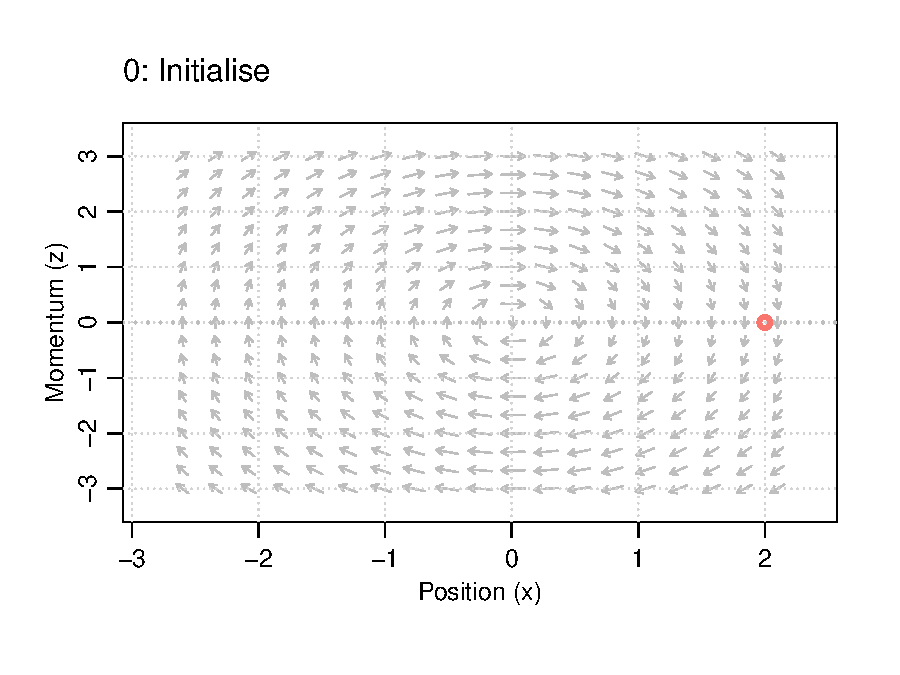
\includegraphics[width=0.49\textwidth]{figure/04-phase1}
  \vspace{-20pt}
  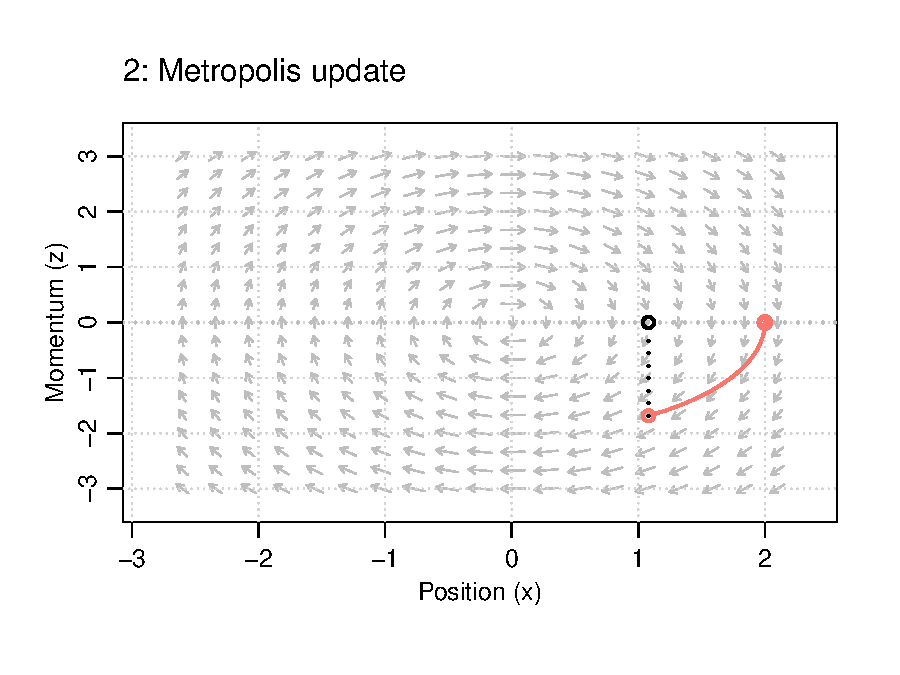
\includegraphics[width=0.49\textwidth]{figure/04-phase2}
  \vspace{-20pt}
  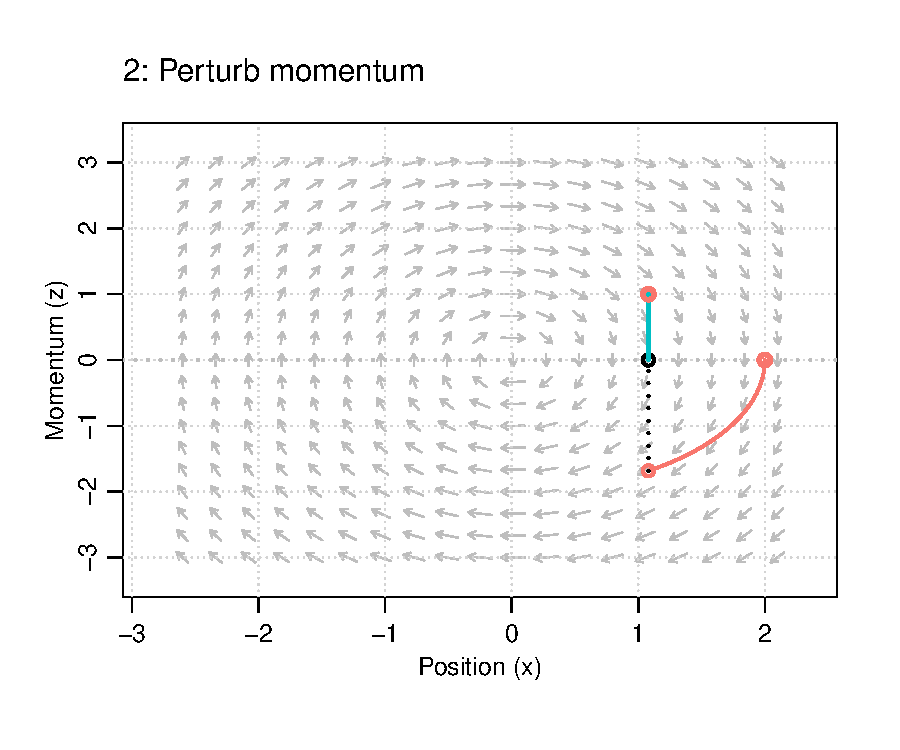
\includegraphics[width=0.49\textwidth]{figure/04-phase3}
  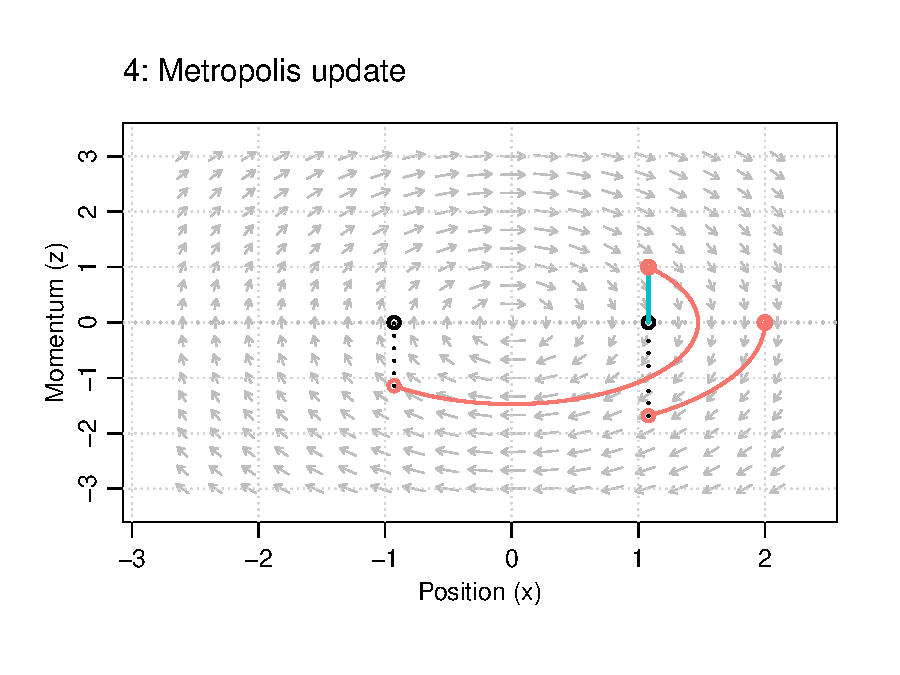
\includegraphics[width=0.49\textwidth]{figure/04-phase4}
  \vspace{-20pt}
  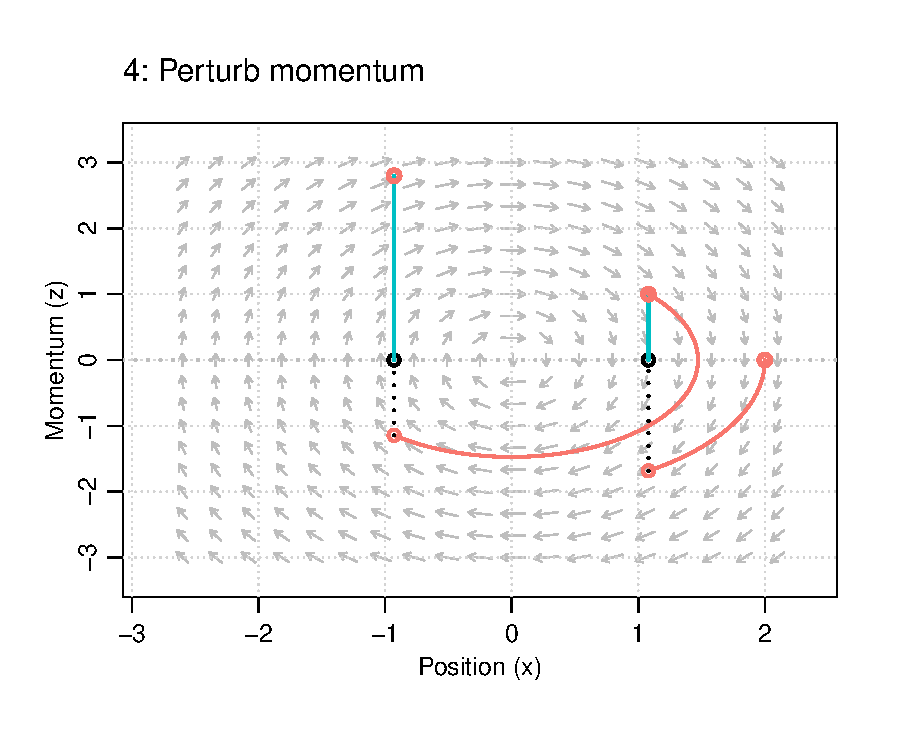
\includegraphics[width=0.49\textwidth]{figure/04-phase5}
  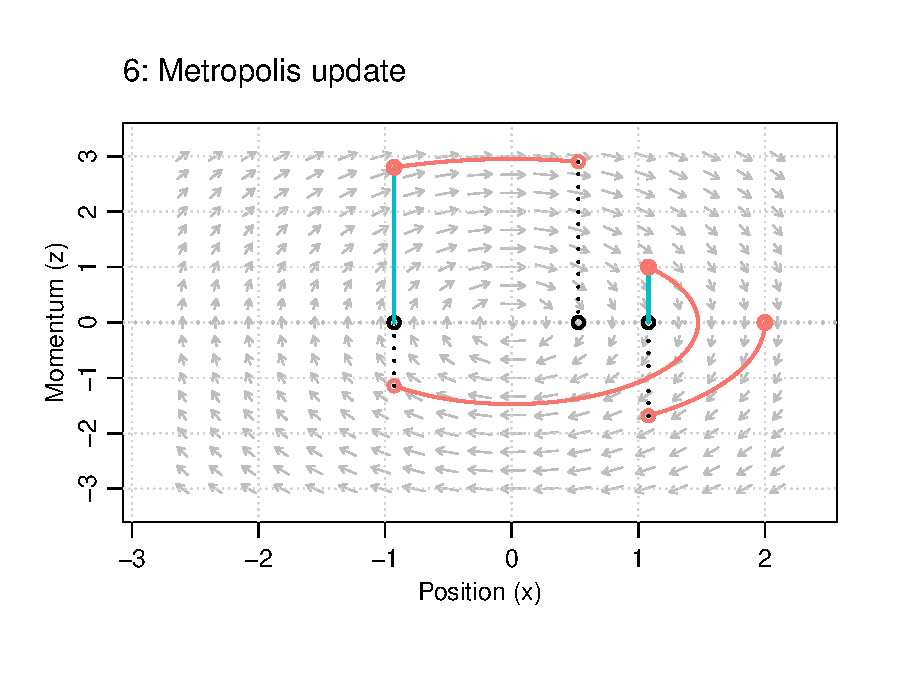
\includegraphics[width=0.49\textwidth]{figure/04-phase6}
  \vspace{-20pt}  
  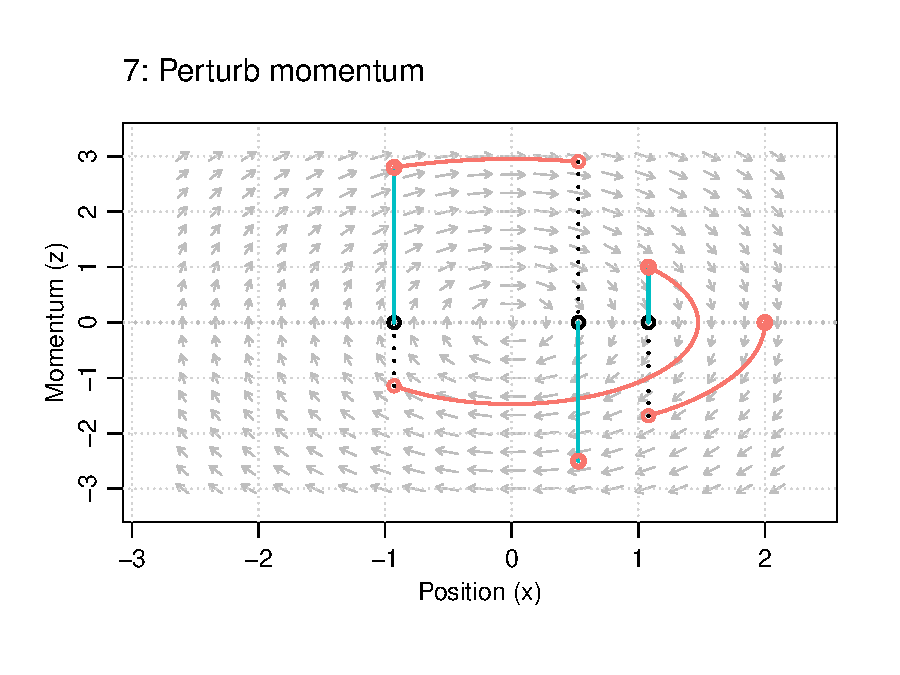
\includegraphics[width=0.49\textwidth]{figure/04-phase7}
  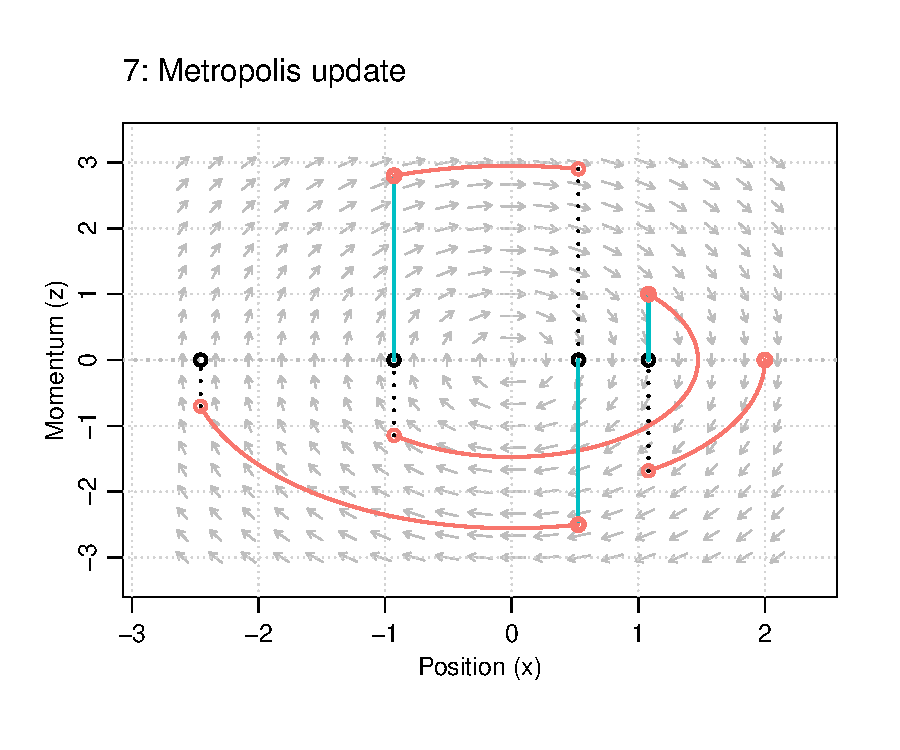
\includegraphics[width=0.49\textwidth]{figure/04-phase8}
  \caption{A phase diagram schematic of HMC sampling in one-dimension. At step 0, initialise values for momentum and position. At step 1, simulate movement using Hamiltonian dynamics, accept position and discard momentum. At step 2, perturb momentum using a normal density, then repeat.}
\end{figure}

HMC is often times superior to standard Gibbs sampling, for a variety of reasons. 
For one, conjugacy does not play any role in the efficiency of the HMC sampler, thus freeing the modeller to choose more appropriate and more intuitive prior densities for the parameters of the model. 
For another, the HMC sampler is designed to incite little autocorrelations between samples, and thus increasing efficiency.

Several drawbacks do exist with the HMC sampler. Firstly, it is impossible to directly sample from discrete distributions $p(x)$.
More concretely, HMC requires that the domain of $p(x)$ is continuous and that $\partial \log p(x) / \partial x$ is inexpensive to compute.
To work around this, one must reformulate the model by marginalising out the discrete variables, and obtain them back later by separately sampling from their posteriors.
Alternatively, a Gibbs sampler specifically for the discrete variables could be augmented with the HMC sampler.
The other drawback of HMC is that there are many tuning parameters (leapfrog $L$, step-size $\epsilon$, mass matrix $M$, etc.)  that is not immediately easy to perfect, at least not to the novice user. 

The implementation of HMC by the programming language \proglang{Stan}, which interfaces many other programming languages including \proglang{R}, \proglang{Python}, \proglang{MATLAB}, \proglang{Julia}, \proglang{Stata} and \proglang{Mathematica}, is a huge step forward in computational Bayesian analysis.
\proglang{Stan} takes the liberty of performing all the tuning necessary, and the practitioner is left with simply specifying the model. 
A vast library of differentiable probability functions are available, with the ability to bring your own code as well.
Development is very active and many improvements and optimisations have been made since its inception.

\footnotetext{Thinking back to elementary mechanics, this is the familiar $\half m v^2$ formula for kinetic energy and substituting in the identity $z =mv$, where $m$ is the mass of the object, and $v$ is its velocity.}

\chapter{Variational inference}
\thispagestyle{chaptersthree}
\index{variational inference}
Consider a statistical model parameterised by $\btheta = (\theta_1,\dots,\theta_p)^\top$ for which we have observations $\by := \{y_1,\dots,y_n\}$, but also some latent variables $\bw$.
Typically, in such models, there is a want to to evaluate the integral 
\begin{equation}\label{eq:varint2} 
  I = \int p(\by|\bw) p(\bw) \dint \bw,
\end{equation}
Marginalising out the latent variables in \cref{eq:varint2} is usually a precursor to obtaining a log-likelihood function to be maximised in a frequentist setting, whereby there is an implicit dependence on the model parameters in the evaluation of $I$.
In Bayesian analysis, priors are specified on the model parameters $\theta\sim p(\theta)$.
By concatenating the latent variables and model parameters to form $\bw$, the $I$ corresponds to the marginal density for $\by$, on which the posterior depends.

In many instances, for one reason or another, evaluation of \cref{eq:varint2} or is difficult, in which case inference is halted unless a way of overcoming the intractability is found.
In this chapter, we discus \emph{variational inference} (VI) as a means of approximating the integral.
The literature on variational inference is typically presented in a Bayesian light \citep{jordan1999introduction,bishop2006pattern,blei2017variational}, and as such, it is commonly known as \emph{variational Bayes} method.
The main attraction from a Bayesian point of view is that it provides a deterministic way of obtaining (approximate) posteriors, i.e. it does not involve sampling from posteriors.

Variational inference can be used in conjunction with an EM algorithm, in which the E-step is replaced with a variational E-step.
This \emph{variational EM algorithm} is used for maximum likelihood learning, but can modified to obtain maximum a posteriori estimates.
In the works of \citep{beal2003variational,beal2003}, the authors realised that the EM algorithm can be extended easily to obtain posterior densities of the latent variables and parameters if the statistical model is conjugate exponential family.
They refer to this as the \emph{variational Bayes EM algorithm}, but in fact this is really just variational inference in which the algorithm resembles an EM algorithm with clear E- and M-steps.

We first briefly introduce variational methods for approximating the intractable integral, and this is usually considered a fully Bayesian treatment of the model.
We then describe variational EM, and provide a comparison of the two methods.

\section{A brief introduction to variational inference}
\label{sec:varintro}






The crux of variational inference is this: find a suitably close distribution function $q(\bw)$ that approximates the true posterior $p(\bw|\by)$, where closeness here is defined in the Kullback-Leibler divergence sense,
\[
  \KL(q\Vert p) = \int \log \frac{q(\bw)}{p(\bw|\by)} q(\bw) \dint \bw.
\]
Posterior inference is then conducted using $q(\bw)$ in lieu of $p(\bw|\by)$.
Advantages of this method are that 1) it is fast to implement computationally (compared to MCMC); 2) convergence is assessed simply by monitoring a single convergence criterion; and 3) it works well in practice, as attested to by the many studies implementing VI.

Briefly, we present the motivation behind variational inference and the minimisation of the KL divergence.
Denote by $q(\cdot)$ some density function of $\bw$.
One may show that log marginal density, i.e. the log of the intractable integral \cref{eq:varint}, holds the following bound:
\begin{align}
  \log p(y) &= \log p(\by,\bw) - \log p(\bw|\by) \mycomment{\footnotesize (Bayes' theorem)} \nonumber \\
  &= \int \left\{ \log \frac{p(\by,\bw)}{q(\bw)} - \log \frac{p(\bw|\by)}{q(\bw)} \right\} q(\bw) \dint \bw \mycomment{\footnotesize (expectation both sides)} \hspace{1cm} \nonumber \\    
  &=  \cL(q) +  \KL(q \Vert p) \nonumber \\
  &\geq \cL(q) \label{eq:varbound}
\end{align}
since the KL divergence is a non-negative quantity.
The functional $\cL(q)$ given by 
\begin{align}
  \cL(q) 
  &= \int \log \frac{p(\by,\bw)}{q(\bw)} q(\bw) \dint \bw \nonumber \\
%  &= \E_{\bw\sim q}[\log p(\by,\bw) - \log q(\bw)] \nonumber \\
  &= \E_{\bw\sim q}[\log p(\by,\bw)] + H(q), \label{eq:elbo1}
\end{align}
where $H$ is the entropy functional, is known as the \emph{evidence lower bound} (ELBO).
Evidently, the closer $q$ is to the true $p$, the better, and this is achieved by maximising $\cL$, or equivalently, minimising the KL divergence from $p$ to $q$.
Note that the bound \cref{eq:varbound} achieves equality if and only if $q(\bw) \equiv p(\bw|\by)$, but of course the true form of the posterior is unknown to us---see \cref{sec:varEM} for a discussion.
Maximising $\cL(q)$ or minimising $\KL(q\Vert p)$ with respect to the density $q$ is a problem of calculus of variations, which incidentally, is where variational inference takes its name.
The astute reader will realise that $\KL(q||p)$ is impossible to compute, since one does not know the true distribution $p(\bw|\by)$. Efforts are concentrated on maximising the ELBO instead.

Maximising $\cL$ over all possible density functions $q$ is not possible without considering certain constraints.
Two such constraints are described. 
The first, is to make a distributional assumption regarding $q$, for which it is parameterised by $\nu$.
For instance, we might choose the closest normal distribution to the posterior $p(\bw|\by)$ in terms of KL divergence.
In this case, the task is to find optimal mean and variance parameters of a normal distribution.

\begin{figure}[htb]
  \centering
  \begin{tikzpicture}
    \draw[ultra thick] (0,0) ellipse (4cm and 2.2cm);
    \node at (-2.8,0.7) {$q(\bw;\nu)$};
    \draw[thick,colred] (-0.8,-0.5) to [curve through={(-2,0) .. (-2,-0.8) .. (1,-0.8) .. (-1,1.5) .. (0,1.5) ..(0.3,0.1) .. (0.5,1.5) .. (2,0) .. (2.1,-0.1) .. (2.2,1.1) .. (3,0.9)}] (3.317,1.225);  % curve using hobby tikz
    \draw[dashed, very thick,black!50] (3.317,1.225) -- (4.05,2.1);
    \fill (-0.8,-0.5) circle (2.2pt) node[below] {$\nu^{\text{init}}$};
    \fill (3.317,1.225) circle (2.2pt) node[left,yshift=-1] {$\nu^*$};
    \fill (4.05,2.1) circle (2.2pt) node[right,yshift=1] {$p(\bw|\by)$};
    \node[gray] at (4.5,1.4) {$\KL(q\Vert p)$};
  \end{tikzpicture}
  \vspace{-1em}
  \caption[Schematic view of variational inference]{Schematic view of variational inference\footnotemark. The aim is to find the closest distribution $q$ (parameterised by a variational parameter $\nu$) to $p$ in terms of KL divergence within the set of variational distributions, represented by the ellipse.}
\end{figure}
\footnotetext{Reproduced from the talk by David Blei entitled ``Variational Inference: Foundations and Innovations'', 2017. URL: \url{https://simons.berkeley.edu/talks/david-blei-2017-5-1}.}

The second type of constraint, and the one considered in this thesis, is simply an assumption that the approximate posterior $q$ factorises into $M$ disjoint factors.
Partition $\bw$ into $M$ disjoint groups $\bw = (w_{[1]},\dots,w_{[M]})$.
Note that each factor $w_{[k]}$ may be multidimensional.
Then, the structure
\[
  q(\bw) = \prod_{k=1}^M q_k(w_{[k]})
\]
for $q$ is considered.
This factorised form of variational inference is known in the statistical physics literature as the \emph{mean-field theory} \citep{itzykson1991statistical}.

\begin{remark}
The choice of factorisation is completely arbitrary, although forcing a factorisation also induces independence between the factors in the posterior, and this may or may not be suitable for the problem at hand.
Landing the correct choice of factorisation is rather experimental, as the aim is to balance tractability and model misspeficication.
In a model with both latent variables and random parameters (in a Bayesian setting), then a good starting point would be to factorise the latent variables and parameters.
\end{remark}

\index{ELBO}
Let us denote the distributions which minimise the Kullback-Leibler divergence (maximise the variational lower bound) by the use of tildes.
The impact of the mean-field factorisation on the ELBO is inspected:
\begin{align*}
  \cL(q) 
  &= \idotsint \log \frac{p(\by,\bw)}{\prod_{k=1}^M q_k(\bw)}  \prod_{k=1}^m \left\{ q_k(w_{[k]}) \dint w_{[k]} \right\} \\
  &= \idotsint \left( \log p(\by,\bw) - \sum_{k=1}^M \log q_k(\bw)  \right) \prod_{k=1}^M \left\{ q_k(w_{[k]}) \dint w_{[k]} \right\} 
\end{align*}
and rearranging slightly for terms involving the $j$'th component only, we get
\begin{align*}
  \cL(q) 
  ={}& \idotsint \left( \log p(\by,\bw)  - \log q_j(w_{[j]}) + \const \right) q_j(w_{[j]}) \dint w_{[j]} \prod_{k\neq j} \left\{ q_k(w_{[k]}) \dint w_{[k]} \right\} \\
  ={}& \int  \Bigg( \,
  \myoverbrace{\idotsint \log p(\by,\bw)  \prod_{k\neq j} \left\{ q_k(w_{[k]}) \dint w_{[k]} \right\}}{\log \tilde p(\by,w_{[j]}) + \const}
  \, \Bigg) q_j(w_{[j]}) \dint w_{[j]} \\
  & - \int  \log q_j(w_{[j]}) q_j(w_{[j]}) \dint w_{[j]} + \const \\
  ={}& -\KL(q_{[j]} \Vert \tilde p) + \const
\end{align*}
The task of maximising $\cL$ is then equivalent to maximising $-\KL(q_{[j]} \Vert \tilde p)$, where $\tilde p$ is defined in the overbrace of the second line in the equation above.
Thus, for each $w_{[k]}$, $k=1,\dots,M$, $\tilde q_k$ satisfies
\begin{align}\label{eq:qtilde}
  \log \tilde q_k(w_{[k]}) = \E_{-k} [ \log p(\by,\bw) ] + \const
\end{align}
where expectation of the joint log density of $\by$ and $\bw$ is taken with respect to all of the unknowns $\bw$, except the one currently in consideration $w_{[k]}$, under their respective $\tilde q_k$ densities. 
For further details, refer to \citet[Eq. 10.9, p. 466]{bishop2006pattern}.

In practice, rather than an explicit calculation of the normalising constant, one simply needs to inspect \cref{eq:qtilde} to recognise it as a known log-density function, which is the case when exponential family distributions are considered.
That is, suppose that each complete conditional $p(w_{[k]}|\bw_{-k}, \by)$, where $\bw_{-k} = \{w_{[i]} \,|\, i \neq k\}$, follows an exponential family distribution
\[
  p(w_{[k]}| \bw_{-k}, \by ) 
  = B(w_{[k]})\exp \big(\ip{\zeta_k(\bw_{-k}, \by) , w_{[k]}} - A(\zeta_k) \big).
\]
Then, from \cref{eq:qtilde},
\begin{align*}
  \tilde q(w_{[k]})
  &\propto \exp \left( \E_{-k} \left[ \log p(w_{[k]}| \bw_{-k}, \by) \right] \right) \\
  &= \exp \Big(\log B(w_{[k]}) + \E \ip{\zeta_k(\bw_{-k}, \by) , w_{[k]}} - \E [ A(\zeta_k) ] \Big) \\
  &\propto B(w_{[k]})\exp \E\ip{\zeta_\xi(\bw_{-k}, \by) , w_{[k]}}
\end{align*}
is also in the same exponential family.
In situations where there is no closed form expression for $\tilde q$, then one resorts to sampling methods such as a Metropolis random walk to estimate quantities of interest.
This stochastic step within a deterministic algorithm has been explored before in the context of a Monte Carlo EM algorithm---see \citet[Sec. 4]{meng1997algorithm} and references therein.

One notices that the optimal mean-field variational densities for each component are coupled with one another, in the sense that the distribution $\tilde q_k$ depends on the moments of the rest of the components $\bw_{-k}$.
For very simple problems, an exact solution for each $\tilde q_k$ can be found, but usually, the way around this is to employ an iterative procedure.
The \emph{coordinate ascent mean-field variational inference} (CAVI) algorithm cycles through each of the distributions in turn, updating them in sequence starting with arbitrary distributions as initial values.
\index{coordinate ascent variational inference (CAVI)}

\algrenewcommand{\algorithmiccomment}[1]{{\color{grymath} \hfill $\triangleright$ #1}}
\begin{algorithm}[H]
\caption{The CAVI algorithm}\label{alg:cavi}
  \begin{algorithmic}[1]
    \State \textbf{initialise} Variational factors $q_k(w_{[k]})$
    \While{ELBO $\cL(q)$ not converged}
      \For{$k = 1,\dots,M$}
        \State $\tilde q_k(w_{[k]}) \gets \const \times \exp \E_{-k}\left[ \log p(\by,\bw) \right]$ \Comment{from \cref{eq:qtilde}}
      \EndFor
      \State $\cL(q) \gets \E_{\bw \sim \prod_k\tilde q_k}\log p(\by, \bw) + \sum_{k=1}^m H\big[ q_k(w_{[k]})\big]$ \Comment{Update ELBO}
    \EndWhile
    \State \textbf{return} $\tilde q(\bw) = \prod_{k=1}^M \tilde q_j(w_{[k]})$ 
  \end{algorithmic}
\end{algorithm}

Each iteration of the CAVI brings about an improvement in the ELBO (hence the name coordinate ascent).
The algorithm terminates when there is no more significant improvement in the ELBO, indicating a convergence of the CAVI.
\citet{blei2017variational} notes that the ELBO is typically a non-convex function, in which case convergence may be to (one of possibly many) local optima.
A simple solution would be to restart the CAVI at multiple initial values, and the solution giving the highest ELBO is the distribution that is closest to the true posterior.

\section{Variational EM algorithm}
\label{sec:varEM}\index{variational EM algorithm}
% https://tex.stackexchange.com/questions/124269/energy-level-diagrams-with-tex
\tikzset{
    level/.style = {
        ultra thick,
    },
    connect/.style = {
        dashed,
        red
    },
    notice/.style = {
        draw,
        rectangle callout,
        callout relative pointer={#1}
    },
    label/.style = {
        text width=2cm
    }
}

\newcommand{\energyem}[1][1.5]{
\begin{tikzpicture}
  % Draw all levels
%  \draw[draw=none] (0, 8/#1) -- node[above] {EM Algorithm} (5, 8/#1);  % new top
  \draw[level,colred] (0, 6.5/#1) -- node[above] {} node[below] {} (5, 6.5/#1);  % top
  \draw[level,colblu] (0, 3.25/#1) -- node[above] {} node[below] {} (2.5, 3.25/#1);  % mid
  \draw[level] (0,0) -- node[above] {} (5, 0);  % bottom
  
  % Draw arrows
  \draw[<->,very thick] (0.75, 3.25/#1) -- node[left] {$\KL(q\Vert p)$} (0.75, 6.5/#1);
  \draw[<->,very thick] (1.75,0) -- node[left] {$\cL(q,\theta)$} (1.75,3.25/#1);
  \draw[<->,very thick] (3.5,0) -- node[right] {$\log p(\by|\theta)$} (3.5,6.5/#1);
\end{tikzpicture}
}

\newcommand{\energyemEstep}[1][2.15]{
\begin{tikzpicture}
  % Draw all levels
  \draw[draw=none] (0,8/#1) -- node[above] {EM (E-step)} (5,8/#1);  % new top
  \draw[level,colred] (0,6.5/#1) -- node[above] {} node[below] {} (5,6.5/#1);  % top
  \draw[level,colblu,dashed] (0,3.25/#1) -- node[above] {} node[below] {} (2.5,3.25/#1);  % mid
  \draw[level] (0,0) -- node[above] {} (5,0);  % bottom
  
  % Draw arrows
  \draw[<->,very thick,opacity=0] (0.75,3.25/#1) -- node[left] {\footnotesize $\KL(q\Vert p)$} (0.75,6.5/#1);
  \draw[<->,very thick] (3.5,0) -- node[right] {\footnotesize $\log p(\by|\theta^{\text{old}})$} (3.5,6.5/#1);
  
  % E-step
  \draw[level,colblu] (0,6.5/#1) -- node[above] {\color{black!99}\footnotesize $ \KL(q^{\text{new}} \Vert p) = 0$} (2.5,6.5/#1);  % top      
  \draw[->,very thick,colblu] (2,3.25/#1) -- node[left] {} (2,6.5/#1);  
  \draw[<->,very thick] (1.25,0) -- node[left,yshift=-33/#1] {\footnotesize $\cL(q^{\text{new}},\theta^{\text{old}})$} (1.25,6.5/#1);      
  
  \draw[white] (0,0) -- (0,-0.5);
\end{tikzpicture}
}

\newcommand{\energyemMstepfade}[1][2.15]{
\begin{tikzpicture}[opacity=0.25]
  % Draw all levels
  \draw[level,colred] (0,8/#1) -- node[above] {\color{black!99} EM (M-step)} (5,8/#1);  % new top
  \draw[level,colblu,dashed] (0,6.5/#1) -- node[above] {} node[below] {} (2.5,6.5/#1);  % mid
  \draw[level,colred,dashed] (2.5,6.5/#1) -- node[above] {} node[below] {} (5,6.5/#1);  % mid
  \draw[level] (0,0) -- node[above] {} (5,0);  % bottom
  \draw[level,colblu] (0,7.1/#1) -- node[above] {} node[below] {} (2.5,7.1/#1);  % mid
  
  % Draw arrows
  \draw[<->,very thick] (0.75,7.1/#1) -- node[left] {\footnotesize $\KL(q^{\text{new}} \Vert p)$} (0.75,8/#1);
  \draw[<->,very thick] (1.25,0) -- node[left] {\footnotesize $\cL(q^{\text{new}},\theta^{\text{new}})$} (1.25,7.1/#1);         
  \draw[<->,very thick] (3.5,0) -- node[right] {\footnotesize $\log p(\by|\theta^{\text{new}})$} (3.5,8/#1);
  \draw[->,very thick,colblu] (2,6.5/#1) -- node[left] {} (2,7.1/#1);  
  \draw[->,very thick,colred] (4.5,6.5/#1) -- node[left] {} (4.5,8/#1);  
  
  \draw[white] (0,0) -- (0,-0.5);
\end{tikzpicture}
}


\newcommand{\energyemMstep}[1][2.15]{
\begin{tikzpicture}
  % Shaded region
  \fill[colred!10] (0,6.5/#1) rectangle (5,8/#1);
  
  % Draw all levels
  \draw[level,colred] (0,8/#1) -- node[above] {\color{black!99} EM (M-step)} (5,8/#1);  % new top
  \draw[level,colblu,dashed] (0,6.5/#1) -- node[above] {} node[below] {} (2.5,6.5/#1);  % mid
  \draw[level,colred,dashed] (2.5,6.5/#1) -- node[above] {} node[below] {} (5,6.5/#1);  % mid
  \draw[level] (0,0) -- node[above] {} (5,0);  % bottom
  \draw[level,colblu] (0,7.1/#1) -- node[above] {} node[below] {} (2.5,7.1/#1);  % mid
  
  % Draw arrows
  \draw[<->,very thick] (0.75,7.1/#1) -- node[left] {\footnotesize $\KL(q^{\text{new}}\Vert p)$} (0.75,8/#1);
  \draw[<->,very thick] (1.25,0) -- node[left] {\footnotesize $\cL(q^{\text{new}},\theta^{\text{new}})$} (1.25,7.1/#1);         
  \draw[<->,very thick] (3.5,0) -- node[right] {\footnotesize $\log p(\by|\theta^{\text{new}})$} (3.5,8/#1);
  \draw[->,very thick,colblu] (2,6.5/#1) -- node[left] {} (2,7.1/#1);  
  \draw[->,very thick,colred] (4.5,6.5/#1) -- node[left] {} (4.5,8/#1);   

  \draw[white] (0,0) -- (0,-0.5);
\end{tikzpicture}
}

\newcommand{\energyvbEstep}[1][2.15]{
\begin{tikzpicture}
  % Draw all levels
  \draw[draw=none] (0,8/#1) -- node[above] {VEM (E-step)} (5,8/#1);  % new top
  \draw[level,colred] (0,6.5/#1) -- node[above] {} node[below] {} (5,6.5/#1);  % top
  \draw[level,colblu,dashed] (0,3.25/#1) -- node[above] {} node[below] {} (2.5,3.25/#1);  % mid
  \draw[level] (0,0) -- node[above] {} (5,0);  % bottom
  
  % Draw arrows
  \draw[<->,very thick] (0.75,5.25/#1) -- node[left] {\footnotesize $\KL(q^{\text{new}} \Vert p)$} (0.75,6.5/#1);
  \draw[<->,very thick] (3.5,0) -- node[right] {\footnotesize $\log p(\by|\theta^{\text{old}})$} (3.5,6.5/#1);
  
  % E-step
  \draw[level,colblu] (0,5.25/#1) -- node[above] {} (2.5,5.25/#1);  % new KL level     
  \draw[->,very thick,colblu] (2,3.25/#1) -- node[left] {} (2,5.25/#1);  % increase in L  
  \draw[<->,very thick] (1.25,0) -- node[left,yshift=-33/#1] {\footnotesize $\cL(q^{\text{new}},\theta^{\text{old}})$} (1.25,5.25/#1);    

  \draw[white] (0,0) -- (0,-0.5);
\end{tikzpicture}
}

\newcommand{\energyvbMstepa}[1][2.15]{
\begin{tikzpicture}
  % Shaded region
  \fill[colred!10] (0,6.5/#1) rectangle (5,8/#1);  
  
  % Draw all levels
  \draw[level,colred] (0,8/#1) -- node[above] {\color{black!99} VEM (M-step)---scenario A} (5,8/#1);  % new top
  \draw[level,colred,dashed] (2.5,6.5/#1) -- node[above] {} node[below] {} (5,6.5/#1);  % top
  \draw[level,colblu] (0,6.5/#1) -- node[above] {} node[below] {} (2.5,6.5/#1);  % top
  \draw[level] (0,0) -- node[above] {} (5,0);  % bottom
  \draw[level,colblu,dashed] (0,5.25/#1) -- node[above] {} (2.5,5.25/#1);  % new KL level     

  % Draw arrows
  \draw[<->,very thick] (0.75,6.5/#1) -- node[left] {\footnotesize $\KL(q^{\text{new}}\Vert p)$} (0.75,8/#1);   
  \draw[<->,very thick] (1.25,0) -- node[left] {\footnotesize $\cL(q^{\text{new}},\theta^{\text{new}})$} (1.25,6.5/#1);                  
  \draw[<->,very thick] (3.5,0) -- node[right] {\footnotesize $\log p(\by|\theta^{\text{new}})$} (3.5,8/#1);
  \draw[->,very thick,colblu] (2,5.25/#1) -- node[left] {} (2,6.5/#1);        
  \draw[->,very thick,colred] (4.5,6.5/#1) -- node[left] {} (4.5,8/#1);  

  \draw[white] (0,0) -- (0,-0.5);
\end{tikzpicture}
}

\newcommand{\energyvbMstepb}[1][2.15]{
\begin{tikzpicture}
  % Shaded region
  \fill[colred!10] (0,6.5/#1) rectangle (5,7.25/#1);  
  
  % Draw all levels
  \draw[draw=none] (0,8/#1) -- node[above] {\color{black} VEM (M-step)---scenario B} (5,8/#1);  % new top
  \draw[level,colred] (0,7.25/#1) -- node[above] {} (5,7.25/#1);  % new top
  \draw[level,colred,dashed] (0,6.5/#1) -- node[above] {} node[below] {} (5,6.5/#1);  % top
  \draw[level,colblu] (0,6/#1) -- node[above] {} node[below] {} (2.5,6/#1);  % top
  \draw[level] (0,0) -- node[above] {} (5,0);  % bottom
  \draw[level,colblu,dashed] (0,5.25/#1) -- node[above] {} (2.5,5.25/#1);  % new KL level     

  % Draw arrows
  \draw[<->,very thick] (0.75,6/#1) -- node[left,yshift=6.5/#1] {\footnotesize $\KL(q^{\text{new}}\Vert p)$} (0.75,7.25/#1);   
  \draw[<->,very thick] (1.25,0) -- node[left] {\footnotesize $\cL(q^{\text{new}},\theta^{\text{new}})$} (1.25,6/#1);                  
  \draw[<->,very thick] (3.5,0) -- node[right] {\footnotesize $\log p(\by|\theta^{\text{new}})$} (3.5,7.25/#1);
  \draw[->,very thick,colblu] (2,5.25/#1) -- node[left] {} (2,6/#1);        
  \draw[->,very thick,colred] (4.5,6.5/#1) -- node[left] {} (4.5,7.25/#1); 
  
  \draw[white] (0,0) -- (0,-0.5);
\end{tikzpicture}
}

\newcommand{\energyvbMstepc}[1][2.15]{
\begin{tikzpicture}
  % Draw all levels
  \draw[draw=none] (0,8/#1) -- node[above] {\color{black} VEM (M-step)---scenario C} (5,8/#1);  % new top
  \draw[level,colred] (0,6.5/#1) -- node[above] {} node[below] {} (5,6.5/#1);  % top
  \draw[level,colblu] (0,5.8/#1) -- node[above] {} node[below] {} (2.5,5.8/#1);  % top
  \draw[level] (0,0) -- node[above] {} (5,0);  % bottom
  \draw[level,colblu,dashed] (0,5.25/#1) -- node[above] {} (2.5,5.25/#1);  % new KL level     

  % Draw arrows
  \draw[<->,very thick] (0.75,5.8/#1) -- node[left] {\footnotesize $\KL(q^{\text{new}}\Vert p)$} (0.75,6.5/#1);   
  \draw[<->,very thick] (1.25,0) -- node[left] {\footnotesize $\cL(q^{\text{new}},\theta^{\text{new}})$} (1.25,5.8/#1);                  
  \draw[<->,very thick] (3.5,0) -- node[right] {\footnotesize $\log p(y|\theta^{\text{new}})$} (3.5,6.5/#1);
  \draw[->,very thick,colblu] (2,5.25/#1) -- node[left] {} (2,5.8/#1);    
  
  \draw[white] (0,0) -- (0,-0.5);  
\end{tikzpicture}
}

Consider again the latent variable setup described in \cref{schap:em}, in which the goal is to maximise the (marginal) log-likelihood of the parameters $\theta$ of the model, after integrating out the latent variables, as given by \cref{eq:varint}.
We will see how the EM algorithm relates to minimising the KL divergence between a density $q(\bw)$ and the posterior of $\bw$, and connect this idea to variational methods.

\begin{figure}[htb]
  \centering
  \energyem 
  \caption[Illustration of the decomposition of the log likelihood.]{Illustration\footnotemark~of the decomposition of the log-likelihood into $\cL(q,\theta)$ and $\KL(q \Vert p)$. The quantity $\cL(q,\theta)$ is a lower bound for the log-likelihood.}
  \label{fig:loglikdecomp}
\end{figure}
\footnotetext{Reproduced from \citet[Fig. 9.11]{bishop2006pattern}.}

As we did in deriving \cref{eq:varbound}, we decompose the (marginal) log-likelihood as
\begin{align*}
  \log p(\by|\theta) &= \log p(\by,\bw|\theta) - \log p(\bw|\by,\theta)  \\
  &= \int \left\{ \log \frac{p(\by,\bw|\theta)}{q(\bw)} - \log \frac{p(\bw|\by,\theta)}{q(\bw)} \right\} q(\bw) \dint \bw  \\    
  &= \myunderbrace{\E_{\bw\sim q} \left[\log \frac{p(\by,\bw|\theta)}{q(\bw)} \right]}{\cL(q,\theta)}
  - \myunderbrace{\E_{\bw\sim q} \left[\log \frac{p(\bw|\by,\theta)}{q(\bw)} \right]}{-\KL(q \Vert p)},
\end{align*}
where $q(\bw)$ is any density function over the latent variables.
This decomposition is shown in \cref{fig:loglikdecomp}.
The interest is then to have a density function $q(\bw)$ which is as close as possible to the true posterior density $p(\by|\bw,\theta)$ in the KL divergence sense.
Since the KL divergence is non-negative, minimising $\KL(q\Vert p)$ is equivalent to maximising $\cL(q,\theta)$.

As a remark, the above line of thought should be familiar as it is the exact same one made for variational inference.
The twist here is that we will peruse a distribution which tightens the lower bound $\cL(q,\theta)$ to the marginal log-likelihood, and this happens when $\KL(q\Vert p)$ is exactly zero, and this in turn happens when $q$ is exactly the true posterior density.
That is, for some parameter value, $\theta = \theta^{(t)}$ say, the solution to
\begin{equation}
  \argmax_q \cL(q,\theta^{(t)})
\end{equation}
is $q^{(t+1)}(\bw) = p(\bw|\by,\theta^{(t)})$, because
\begin{align*}
  \KL(q \Vert p) = \E \left[\log \frac{p(\bw|\by,\theta^{(t)})}{p(\bw|\by,\theta^{(t)})} \right] = 0.
\end{align*}
At this stage, we have the equality
\begin{align}
  \log p(\by|\theta) 
  &= \cL(q^{(t+1)},\theta) \\
  &= \E_{\bw\sim q^{(t+1)}} \left[\log \frac{p(\by,\bw|\theta)}{p(\bw|\by,\theta^{(t)})}  \right]  \\
  &= \myunderbrace{\E_{\bw\sim q^{(t+1)}} \big[\log p(\by,\bw|\theta)  \big]}{Q(\theta|\theta^{(t)})}
  - \myunderbrace{\E_{\bw\sim q^{(t+1)}} \big[\log p(\bw|\by,\theta^{(t)})\big]}{-H(q^{(t+1)})},
\end{align}
%for which increasing the value of $\cL(q^{(t+1)},\theta)$ with respect to $\theta$ will bring about an increase in the log-likelihood.

The term on the left is recognised as the $Q$ function of the E-step
\[
  Q(\theta) = Q(\theta|\theta^{(t)}) = \E_\bw\left( \log p(\by,\bw|\theta) \,\big|\, \by,\theta^{(t)} \right),
\]
while the term on the left is an entropy term which does not depend on $\theta$.
Thus, minimising the KL divergence, or maximising the lower bound $\cL$ with respect to $q$, corresponds to the E-step in the EM algorithm.

Furthermore, since equality between the log-likelihood and the lower bound is achieved after the E-step, increasing $\cL(q^{(t+1)},\theta)$ with respect to $\theta$ is sure to bring about an increase in the log-likelihood.
That is, for any $\theta$, we find that
\begin{align*}
  \log p(\by|\theta) - \log p(\by|\theta^{(t)}) 
  &= Q(\theta|\theta^{(t)}) - Q(\theta^{(t)}|\theta^{(t)}) + \Delta \, \text{entropy} \\
  &\geq Q(\theta|\theta^{(t)}) - Q(\theta^{(t)}|\theta^{(t)}).
\end{align*}
because entropy differences are positive by Gibbs' inequality.
We see that maximising $Q$ with respect to $\theta$ (the M-step) brings about an improvement to the log-likelihood value.

To summarise, given initial values $q^{(0)}$ for the distribution  and $\theta^{(0)}$ for the parameters, the EM algorithm is seen as iterating between
\begin{itemize}
  \item \textbf{E-step}: $q^{(t+1)} \gets \argmax_q \cL(q,\theta^{(t)})$, i.e., maximise $\cL(q,\theta)$ with respect to $q$, keeping $\theta$ fixed. This is equivalent to minimising the KL divergence $\KL(q\Vert p)$.
  \item \textbf{M-step}. $\theta^{(t+1)} \gets \argmax_\theta \cL(q^{(t+1)},\theta)$, i.e., maximise $\cL(q,\theta)$ with respect to $\theta$, keeping $q(\bw)$ fixed.
\end{itemize}

When the true posterior distribution $p(\bw|\by)$ is not tractable, then the E-step becomes intractable as well.
By constraining the maximisation in the E-step to consider $q$ belonging to a family of tractable densities, the E-step yields a variational approximation $\tilde q$ to the true posterior.
In \cref{sec:varintro}, we saw that constraining $q$ to be of a factorised form, then $\tilde q$ is a mean-field density.
After a variational E-step, the M-step proceeds as normal.
This form of the EM is known as \emph{variational EM algorithm} (VEM) \citep{beal2003variational}.
The variational EM algorithm can also be modified to obtain MAP estimates by including the log prior density to the maximisation objective in the M-step.

\begin{figure}[p]\label{fig:emVSvem}
  \centering
  \energyemEstep \hspace{0.5cm}
  \energyvbEstep
  \energyemMstep \hspace{0.5cm}
  \energyvbMstepa
  \energyemMstepfade \hspace{0.5cm}
  \energyvbMstepb
  \energyemMstepfade \hspace{0.5cm}
  \energyvbMstepc
  \vspace{-0.5em} 
  \caption[Illustration of EM vs Variational EM algorithms]{Illustration of EM vs Variational EM (VEM) algorithms. Whereas the EM guarantees an increase in log-likelihood value (red shaded region), the VEM does not.}
\end{figure}

Due to an approximation to the true posterior being used in the E-step, there is no guarantee that the log-likelihood value will increase at each iteration.
This is seen pictorially in \cref{fig:emVSvem}: since the bound on the log-likelihood is not tight, increasing this bound will not necessarily cause an increase in log-likelihood value (Scenario C), and even if it did, it may not give as much an increase as it would under the true posterior density (Scenario B).
Scenario A depicts an ideal case whereby the increase in log-likelihood is as much as it would be if the true posterior density was used.

On a practical note, if the posterior density is intractable, then so is the marginal likelihood, which means that we're unable to determine convergence of the EM using the log-likelihood.
Instead, the lower bound $\cL(q,\theta)$ should be used, which monotonically increases to a local optima (as in the CAVI algorithm).

\section{Comparing variational inference and variational EM}

Variational inference is a fully Bayesian treatment of the model, for which the goal is to obtain approximate posterior densities for all latent variables and parameters.
Variational EM algorithm on the other hand has the objective of obtaining ML or MAP estimates of the parameters using an EM algorithm in which the E-step is replaced with a variational E-step.
In some cases, the CAVI algorithm can resemble an EM algorithm, especially when there is a distinction between latent variables and parameters, and a conjugate exponential family model is involved \citep{blei2017variational}.

Variational inference can yield exactly similar point estimates as variational EM if the approximate posterior is symmetric, e.g. a normal distribution.
Under a normal posterior, its mean is used as a point estimate, which coincides with the mode, which is a MAP estimate, or in the case of diffuse priors, a ML estimate.
However, since the output of variational inference are posterior densities instead of a single point estimate, one is able to obtain posterior standard deviations or credibility intervals about the parameters, something which is not so straightforward under a variational EM or even EM framework.

Derivation of the CAVI algorithm and ELBO for specific models is certainly more tedious than the derivation of the variational EM algorithm.
Often, quantities that are required in the derivation include $\E(\theta)$, $\E(\theta^2)$, $\E(\theta^{-1})$, $\E(\log \theta)$ or any other moment of some function of $\theta$, where expectations are taken under the approximating $q$ posterior density.
For certain distributions $q(\theta)$ these quantities can be awkward to compute, and may need approximating themselves.

The computational time and storage requirements of variational methods is virtually the same as EM algorithm \citep{beal2003variational,blei2017variational}.
Consider the mean-field variational approximation.
In variational inference or variational EM, the updating step for the factors involve
\begin{equation}\label{eq:viEstep1}
  \tilde q_k^{(t+1)}(w_{[k]}) \gets \const \times \exp \left( \E_{\bw_{-k}\sim\tilde q^{(t)}}[\log p(\by,\bw)]\right),
\end{equation}
for each of the factors of the approximate posterior $q(\bw) = \prod_{k=1}^M q_k(w_{[k]})$.
In the EM algorithm E-step, one obtains the $Q$ function
\begin{equation}\label{eq:emEstep1}
  Q(\theta|\theta^{(t)}) = \E_{\bw}\big( \log p(\by,\bw)|\by,\theta^{(t)} \big).
\end{equation}
We can see that in both equations \cref{eq:viEstep1} and \cref{eq:emEstep1}, there is a need to compute the expectation of the joint log density, but the difference between the variational inference and EM or variational EM lies in the M-step.
In variational inference one seeks a distribution, while in EM or variational EM one seeks a point estimate (posterior mode) of this distribution.

{\renewcommand{\arraystretch}{1.5}
\begin{table}[]
\centering
\caption{Comparison between variational inference and variational EM.}
\label{tab:vivemcompare}
\begin{tabular}{p{6.5cm}p{6.5cm}}
\toprule
Variational inference & Variational EM\\ 
\midrule
\textbf{GOAL}: Posterior densities for $(\bw, \theta)$                                                          
& \textbf{GOAL}: ML/MAP estimates for $\theta$ \\
Variational approximation for latent variables and parameters $q(\bw,\theta)\approx p(\bw,\theta|\by)$ 
& Variational approximation for latent variables only $q(\bw)\approx p(\bw|\by)$ \\
Priors required on $\theta$                                                                            
& Priors not necessary for $\theta$ \\
Derivation can be tedious 
& Derivation less tedious \\
Inference on $\theta$ through posterior density $q(\theta)$
& Asymptotic distribution of $\theta$ not well studied; standard errors for $\theta$ not easily obtained \\
Suited to conjugate exponential family models: posteriors will be easily recognisable
& Suited to conjugate exponential family models, but not necessary \\
\bottomrule
\end{tabular}
\end{table}
}





%\chapter{componentwise derivative in infinite-dimensional vector spaces}\label[supchap]{misc:comwiseder}
%

Let $\cX$ be a topological vector space, and $g:\cX\to\bbR$ a real-valued function over $\cX$.
Also suppose that $\{e_1,e_2,\dots\}$ is an (algebraic) orthonormal basis for $\cX$, such that any $x\in\cX$ can be represented as $x = x_1e_1 + x_2e_2 + \cdots = (x_1,x_2,\dots)$.
We define the partial derivative of $g$ with respect to the $k$'th component of $x$ as
\[
  \frac{\partial g(x)}{\partial x_k}  = \lim_{t\to 0} \frac{g(x_1,\dots,x_k+t,\dots) - g(x_1,x_2,\dots)}{t}.
\]
Incidentally, this definition also coincides with the Gâteaux derivative of $g$ at $x$ in the direction $e_k$, i.e., $\frac{\partial g(x)}{\partial x_k} = \partial_{e_k}g(x)$.
Denote by 
\[
  \nabla g(x) = \left(
  \frac{\partial g(x)}{\partial x_1}, 
  \frac{\partial g(x)}{\partial x_2},
  \dots
  \right)
\]
the total differential, or as it is more commonly known, the gradient of $g$ at $x$.
This is, in essence, a component-wise derivative of $g$ using the usual definition of derivatives.
The issue here is that the existence of the limits for each component of the differential does not guarantee existence of the gradient.
This is because component-wise convergence does not guarantee convergence with respect to the actual topology of the  space.

\begin{example}[Existence of partial derivatives does not imply differentiability]
Define $g:\bbR^2\to\bbR$ by
\[
  g(x) = 
  \begin{cases}
    \displaystyle\frac{x_1x_2}{x_1^2 + x_2^2} &\text{if } (x_1,x_2) \neq (0,0) \\
    0 &\text{if } x_1=x_2=0.
  \end{cases}
\]
We note that $\lim_{x\to 0} g(x) = \half \neq 0 = g(0,0)$ along the line $x_1 = x_2$.
Therefore, this function is discontinuous, and hence non-differentiable, at zero.
On the other hand, the partial derivatives of $g$ are 
\[
  \frac{\partial g(x)}{\partial x_1} = \frac{x_2(x_2^2-x_1^2)}{(x_1^2+x_2^2)^2}
  \hspace{0.5cm}\text{and}\hspace{0.5cm}
  \frac{\partial g(x)}{\partial x_2} = \frac{x_1(x_1^2-x_2^2)}{(x_1^2+x_2^2)^2},
\]
and thus along the $x_1$-axis, $\frac{\partial g(x_1,0)}{\partial x_1} = 0$, and similarly along the $x_2$-axis, $\frac{\partial g(0,x_2)}{\partial x_2} = 0$.
Existence of partial derivatives is not sufficient in this case for the existence of the gradient.

\end{example}


\hClosingStuffStandalone
\end{document}